%\documentclass[12pt, oneside, margin=2.5cm]{article} 
\documentclass[12pt,openany, oneside,
 article, 
 a4paper, hyphens, english, brazil]{abntex2}
\usepackage{mathptmx}     
\usepackage{geometry}  
\usepackage[utf8]{inputenc}
\usepackage[T1]{fontenc}
\usepackage{lmodern}			% Usa a fonte Latin Modern			

%---- Fonte times new roman
%\usepackage{newtxtext,newtxmath}
%\usepackage{times}
%----

\usepackage{indentfirst}	
\usepackage{csquotes}
\usepackage[brazil]{babel}                     
\usepackage{hyperref}  			% controla a formação do índice
\usepackage{parskip}			% espaçamento entre os parágrafos
\usepackage{microtype} 			% para melhorias de justificação
\usepackage[table,xcdraw]{xcolor}% http://ctan.org/pkg/xcolor
\usepackage{url}
\usepackage{amsfonts}
\usepackage{amsmath}
\usepackage{mathtools}
\usepackage{enumitem}
\usepackage[font=small,labelfont=bf]{caption}
\usepackage{color}
\geometry{a4paper}        
\usepackage{booktabs}   
\usepackage{pgfgantt}
\usepackage{multicol}
\usepackage{stfloats}
\usepackage{booktabs,tabularx}


% ---- BIBLIOGRAFIA ----
%\input{bib}
%\usepackage[brazilian,hyperpageref]{backref}	 % Paginas com as citações na bibl
\usepackage[alf,
doi=true,
abnt-emphasize=bf, 
abnt-thesis-year=both, 
%abnt-repeated-author-omit=yes, 
abnt-last-names=abnt, 
abnt-etal-cite=2, 
abnt-etal-list=5, 
%abnt-etal-text=default, 
abnt-and-type=e, 
abnt-doi=doi
%abnt-url-package=none, 
%abnt-verbatim-entry=no
]{abntex2cite}

%\newcommand{\parencite}[1]{\cite{#1}}

\newcommand{\parencite}{\cite}

%\usepackage{titlesec}

%\titleformat*{\subsection}{\large\bfseries}

\usepackage{tikz}
\usetikzlibrary{shapes,arrows,positioning, calc}

\DeclareMathOperator*{\argmax}{arg\,max}
%\DeclareMathOperator*{\min}{min}
%\DeclareMathOperator*{\max}{max}


%\appto{\bibfont}{\footnotesize}
%\appto{\bibsetup}{\raggedright}
%\renewcommand*{\bibfont}{\small}
%\newcommand{\ra}[1]{\renewcommand{\arraystretch}{#1}}

% \renewcommand{\baselinestretch}{1.5cm} 
 
\titulo{Single Image Haze Removal Using Dark Channel Prior}
%\subtitulo{Implementação da técnica em C++}
\autor{Vinicius Pavanelli Vianna}
\data{2017}
\local{Ribeirão Preto - SP}
\tipotrabalho{Implementação em C++}

\instituicao{%
	UNIVERSIDADE DE SÃO PAULO
	\par
	FFCLRP - DEPARTAMENTO DE FÍSICA
	\par
PROGRAMA DE PÓS-GRADUAÇÃO EM
\par
FÍSICA APLICADA À MEDICINA E BIOLOGIA (FAMB)}

\preambulo{Implementação em C++}


\makeatletter
\hypersetup{
	%pagebackref=true,
	pdftitle={\@title}, 
	pdfauthor={\@author},
	pdfsubject={\imprimirpreambulo},
	pdfcreator={LaTeX with abnTeX2 on TeXstudio},
%	pdfkeywords={Alvenaria estrutural. }{Alvenaria armada. }{Barras. }{Molas helicoidais. }, 
	colorlinks=true,       		% false: boxed links; true: colored links
	linkcolor=black,          	% color of internal links
	citecolor=black,        		% color of links to bibliography
	filecolor=magenta,      		% color of file links
	urlcolor=blue,
	bookmarksdepth=4,
	allcolors=black
}
\makeatother

\makeindex


%\linespread{1.5}
\begin{document}
	\selectlanguage{brazil}
%	\pretextual
	\frenchspacing 

%\imprimircapa

\imprimirfolhaderosto

		\newpage
		
%		\pdfbookmark[0]{\contentsname}{toc}%
%		\tableofcontents*
%		\cleardoublepage
		
	\setcounter{page}{1}
	
	\textual
%	\newpage
%		\pagestyle{empty}
	\pagestyle{plain}
	
\begin{resumo}
	Este documento relata a implementação na linguagem C++ do algoritmo de ``Remoção de névoa em imagens únicas utilizando a precedência do canal escuro'' (em inglês, \textit{Single Image Haze Removal Using Dark Channel Prior}), publicado por Kaiming He, Jian Sun, e Xiaoou Tang em \cite{HazeRemoval}, para apresentação na disciplina de Processamento e Análise de Imagens Médicas do departamento de Física Aplicada à Medicina e Biologia da Faculdade de Filosofia, Ciências e Letras de Ribeirão Preto da Universidade de São Paulo.
	
\end{resumo}	
	
\section{Introdução}
\setlength{\ABNTEXcitacaorecuo}{0.9cm}

A importância do estudo do fênomeno da névoa em imagens pode ser descrito muito bem pelo texto feito pelos autores do paper:
\begin{citacao}
Imagens feitas em ambientes externos são normalmente degradadas pelo meio turvo (e.g. partículas e pequenas gotas de água) na atmosfera. Neblina, névoa e fumaça causam este tipo de fenômeno pela absorção atmosférica e seu espalhamento. A irradiância recebida pela câmera de cada ponto da cena é atenuada ao longo da linha de visão. Além disto a luz recebida é mesclada com a luz ambiente refletida na linha de visão pelas partículas atmosféricas. As imagens degradadas perdem contraste e fidelidade de cor. Como a quantidade de espalhamento depende da distância dos pontos da cena até a câmera, a degradação varia espacialmente. 

Remoção da névoa (``haze removal'') é desejada em fotografia computacional, doméstica e aplicações de visão computacional. Em primeiro lugar, remover a névoa aumenta significativamente a visibilidade da cena e corrige o desvio de cor causado pela luz ambiente, geralmente imagens livres de névoa são visualmente mais agradáveis. Em segundo lugar, a maioria dos algoritmos de visão computacional, desde análise de imagem de baixo-nível até reconhecimento de objetos de alto-nível, normalmente assumem que a imagem de entrada (após a calibração radiométrica) é a radiância da cena. A performance de muitos algoritmos de visão (e.g. detecção de elementos, filtros e análise fotométrica) irão inevitavelmente sofrer com radiâncias das cenas desviadas e com baixo contraste. Por último, remover a névoa pode fornecer informações sobre a profundidade e beneficiar muitos algoritmos de visão computacional e edição avançada de imagens. Névoa ou neblina podem ser uma dica muito útil para entender a profundidade da cena. Assim, uma imagem ruim por causa da névoa pode ser aproveitada.
\cite[nossa tradução]{HazeRemoval}
\end{citacao}

\section{Base teórica}
O fenômeno de névoa em imagens é amplamente modelado na área de visão computacional como:
\begin{equation} \label{eq:1}
I(x) = J(x)t(x) + A(1 - t(x))
\end{equation}
Aonde $I(x)$ é a intensidade observada, $J(x)$ é a radiância original da cena, $A$ é a luz atmosférica e $t(x)$ é a transmissão do meio pela qual a luz passou. O propósito da remoção de névoa é conseguir recuperar a função $J(x)$ a partir da imagem capturada pela câmera, $I(x)$.

Para realizar este propósito de recuperar a função $J(x)$, os autores usaram a descoberta deles chamada de ``precedência do canal escuro'' (em inglês, \textit{dark channel pior}), que implica que normalmente as imagens de boa qualidade e sem uma área grande de branco (e.g. sem captar o céu com nuvens brancas ou neve), possui um canal escuro quase que totalmente escuro, como se pode ver na Figura \ref{dark_channels}:

\begin{figure}[htb]
	\caption{\label{fig_circulo}Várias imagens sem névoa com seus canais escuros na esquerda e imagem com névoa (haze) e seu respectivo canal escuro}
	\begin{center}
		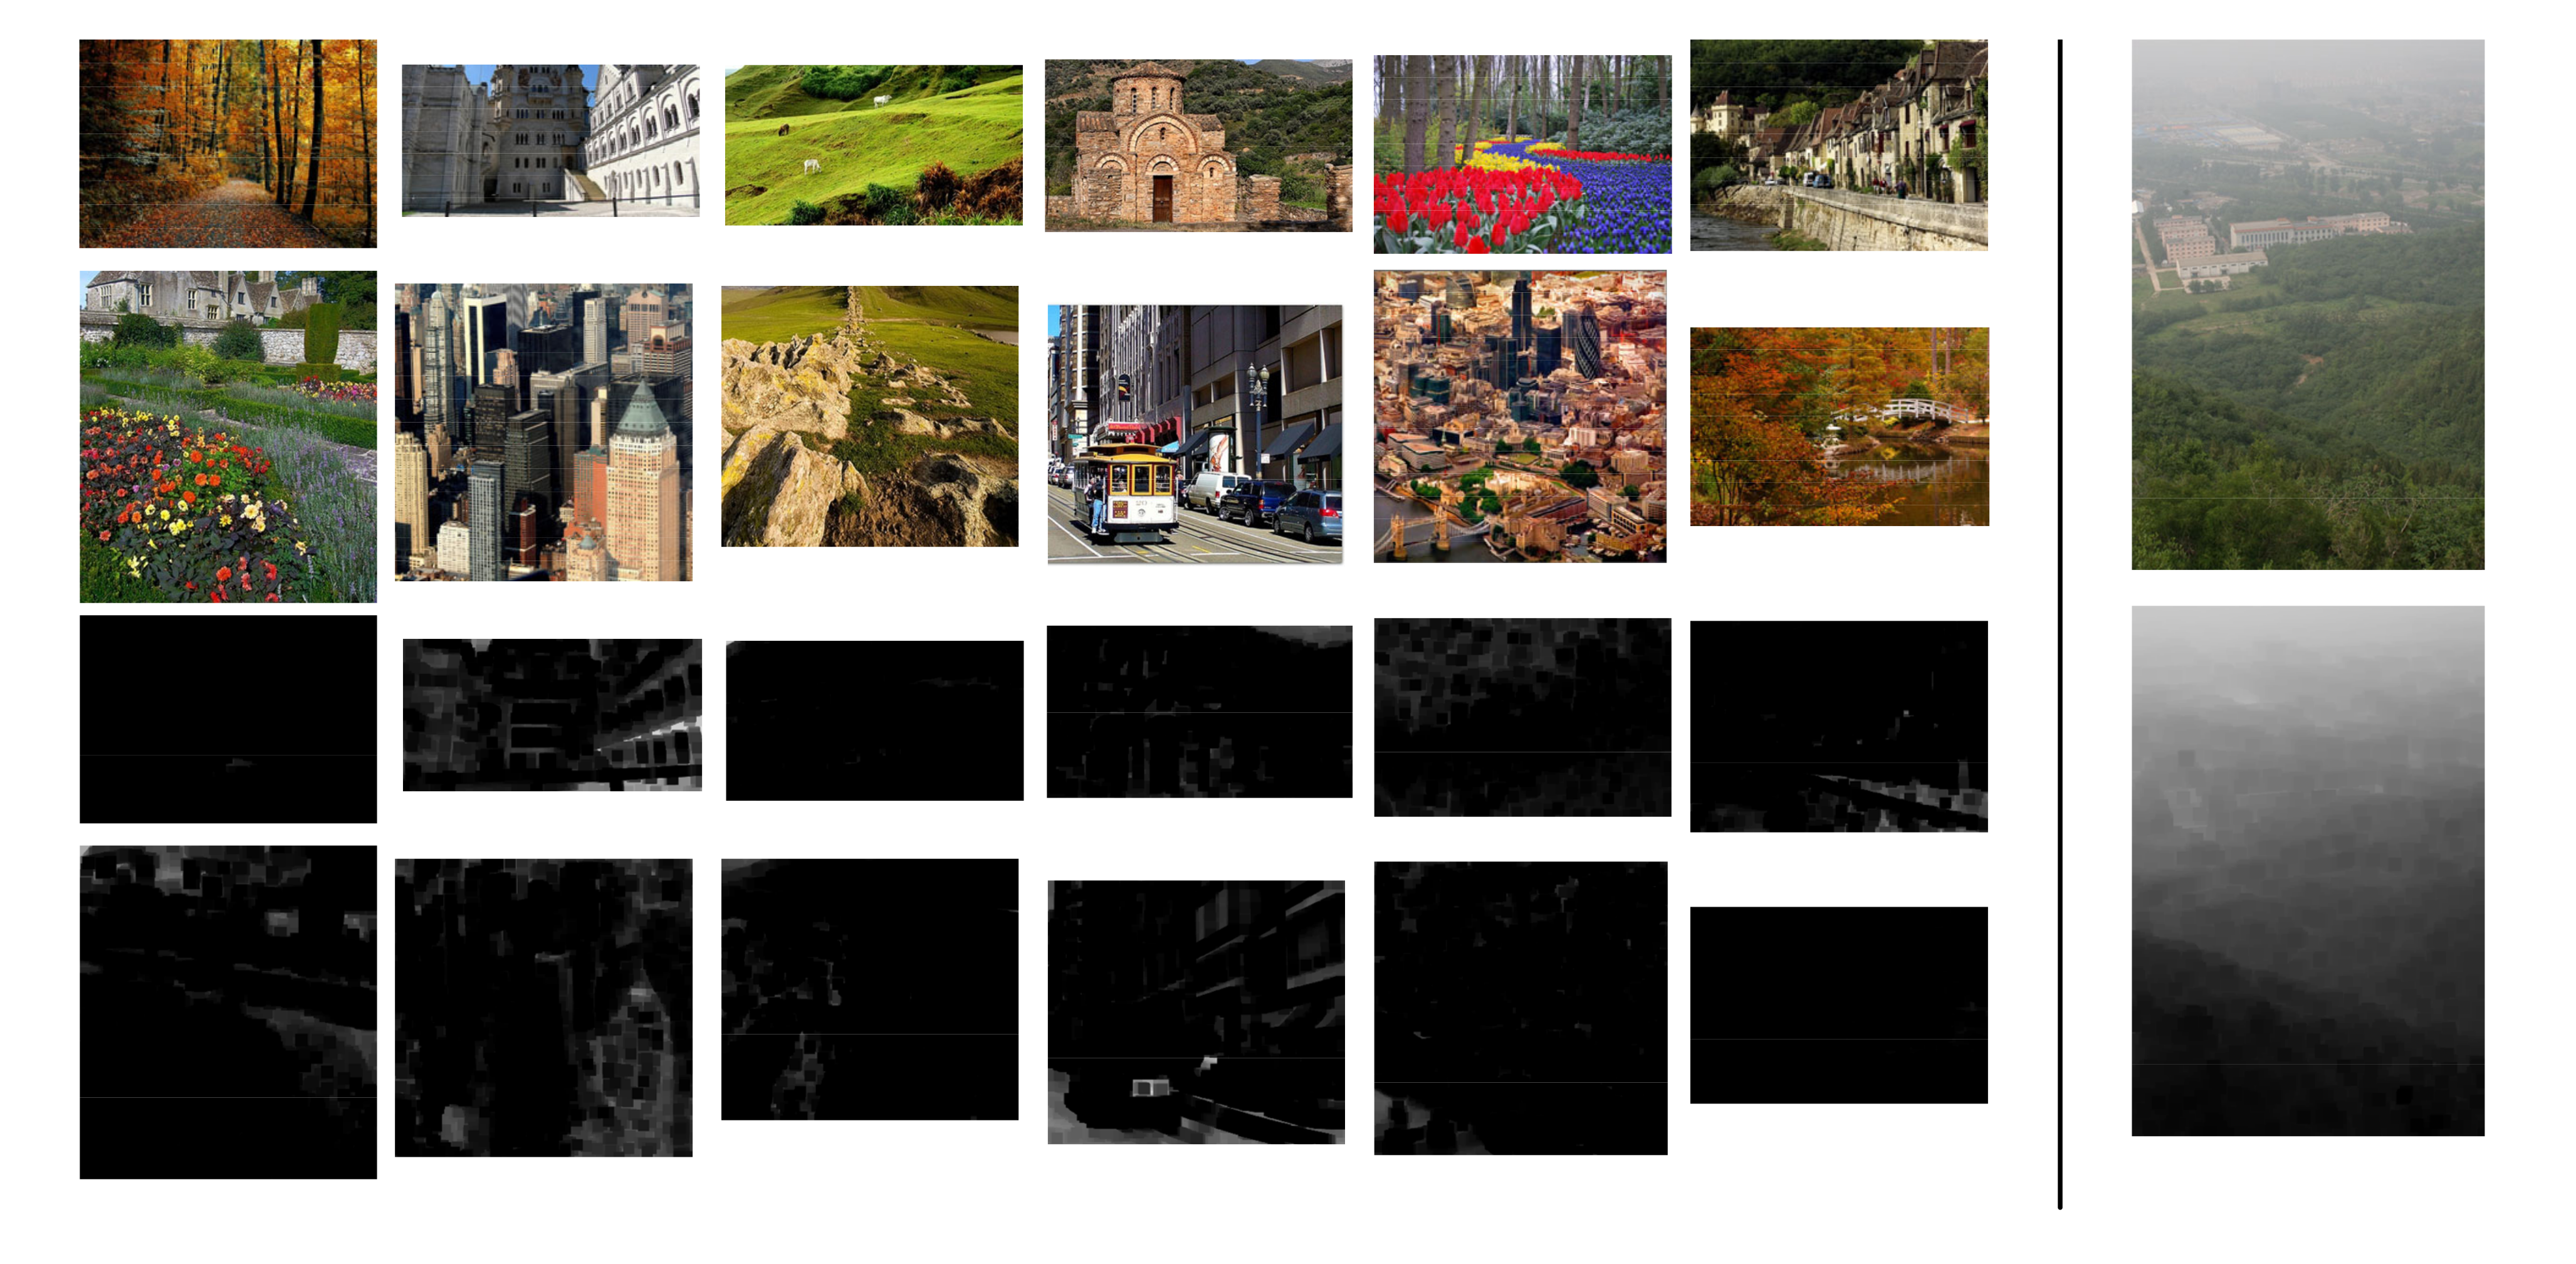
\includegraphics[scale=0.75]{texfiles/dark_channels.png}
	\end{center}
	\legend{Fonte: \cite{HazeRemoval}}
	\label{dark_channels}
\end{figure}

O canal escuro de uma imagem colorida $J^c(x)$ é dado por:
\begin{equation}
J^{dark}(x) = \displaystyle \min_{y \in \Omega(x)} ( \min_{r \in (r,g,b)} J^c(x))
\end{equation}

Aonde $J^c(x)$ é a imagem colorida com seus três componentes RGB, aonde aplicamos o operador $\displaystyle \min_{r \in (r,g,b)}$ para obter o valor mínimo entre esses três componentes e depois aplicamos o operador $\displaystyle \min_{y \in \Omega(x)}$ para obter o valor mínimo do operador anterior dentro de uma janela $\Omega$, no paper estudado esta janela $\Omega$ foi definida como uma janela de $15\times15$ pixels.

O primeiro passo do algoritmo para remover a névoa é normalizar a equação \ref{eq:1} utilizando o valor da luz atmosférica com componentes coloridos $A^c$, gerando a equação:
\begin{equation}\label{eq:3}
\frac{I(x)}{A^c} = \frac{J(x)}{A^c}t(x) + 1 - t(x)
\end{equation}
Depois tomamos o canal escuro de ambos os lados da equação \ref{eq:3}, fazendo a assunção de que a transmissão do meio dentro da uma janela $\Omega$ é constante, gerando uma função de transmissão $\tilde{t}(x)$, que por ser constante pode ser colocado de fora do operado $\min$, e desenvolvendo com a propriedade do canal escuro $J^{dark}(x) \to 0$:
\begin{equation}\label{eq:4}
\begin{gathered}
\displaystyle \min_{y \in \Omega(x)} ( \min_{r \in (r,g,b)} \frac{I(y)}{A^c}) = 
\tilde{t}(y)\displaystyle \min_{y \in \Omega(x)} ( \min_{r \in (r,g,b)} \frac{J(y)}{A^c}) + 1 - \tilde{t}(x)
\\
\displaystyle \min_{y \in \Omega(x)} ( \min_{r \in (r,g,b)} \frac{J(y)}{A^c}) \to 0
\\
\tilde{t}(x) = 1 - \displaystyle \min_{y \in \Omega(x)} ( \min_{r \in (r,g,b)} \frac{I(y)}{A^c}) = 1 - J^{dark}(x)
\end{gathered}
\end{equation}

Para uma melhoria desta função de transmissão $\tilde{t}(x)$ encontrada na equação \ref{eq:4}, o autor utilizada a propriedade chamada ``soft matting'' ou ``image matting'' (tecedor de imagens, nossa tradução), publicado em \cite{matting}, que tem uma equação bem semelhante à equação \ref{eq:1}, e portanto uma solução igual:
\begin{equation}\label{eq:5}
I = F\alpha + B(1-\alpha)
\end{equation}
Aonde $F$ é o canal do primeiro plano, $B$ o canal do fundo e $\alpha$ é a opacidade do primeiro plano. O mapa de transmissão procurado, $t(x)$ é exatamente o $\alpha$ da equação \ref{eq:5}, que pode ser finalmente encontrado utilizando a solução dada por \cite{matting} que consiste em resolver o sistema linear abaixo com uma matriz $L$, chamada de ``matting laplacian'', de tamanho $N \times N$ aonde $N$ é o número de pixels da imagem:
\begin{equation}
\begin{gathered}
(L + \lambda U)t = \lambda \tilde{t}\\
\\
L_{ij} = \displaystyle \sum_{k | (i,j) \in w_k} \left( \delta_{ij} - \frac{1}{|w_k|} \left( 1 + (I_i - \mu_k)^T (\Sigma_k + \frac{\epsilon}{|w_k|}U_3)^{-1}(I_j - \mu_k) \right) \right)
\end{gathered}
\end{equation}
Aonde $L_{ij}$ é o elemento da matriz $L$ na linha $i$, coluna $j$, referente aos pixels $i$ e $j$ da imagem; $w_k$ é a janela $3 \times 3$ centrada no pixel $k$; $|w_k|$ é o tamanho da janela, no caso o número $9$; $\delta_{ij}$ é o delta de Kronecker; $\mu_k$ é a média dos pixels dentro da janela $w_k$; $\Sigma_k$ é uma matriz de covariância $3\times3$ dos elementos dentro da janela $w_k$; $U_3$ é a matriz identidade $3\times3$; $I_i$ e $I_j$ são os vetores dos valores RGB dos pixels $i$ e $j$ respectivamente. A somatória de $L_{ij}$ deve ser feita para todas as janelas $w_k$ que contenham os pixels $i$ e $j$, conforme a notação. Os parâmetros $\epsilon$ e $\lambda$ definem a forma como a função $t(x)$ irá seguir a imagem original ou irá se manter como a função inicial $\tilde{t}(x)$, sendo utilizados em \cite{HazeRemoval} os valores: $\epsilon=10^{-4}$ e $\lambda=10^{-4}$.

Com esta solução do mapa de transmissão $t(x)$, a radiância original da cena pode ser encontrada pela equação abaixo, que ainda é limitada por um fator $t_0 = 0,1$ definido no paper original de modo a evitar o ruído gerado pelo processo de recuperação:
\begin{equation}
J(x) = \frac{I(x)-A}{max(t(x), t_0)} + A
\end{equation}
O valor da luz atmosférica $A$ ou $A_c$ pode ser estimado, se não for fornecido inicialmente, utilizando um método proposto também em \cite{matting}, aonde são selecionados os $0,1\%$ pixels mais claros dentro do canal escuro $J^{dark}$ calculado, e então se encontra o pixel mais claro na imagem original, dentro desses pixels encontrados no canal escuro, este pixel mais claro será a estimativa da luz atmosférica $A$.

Um outro método para obter o mapa de transmissão $t(x)$ a partir de $\tilde{t}(x)$ e $I(x)$ foi proposto pelos mesmos autores em \cite{guided_filtering}, que tem a vantagem de ser muito mais eficiente, não acarretando mais na solução da matriz esparsa $L$ mas sim em um método direto que tem complexidade computacional da ordem de $O(N)$, dado pelo algoritmo:

\begin{tabularx}{\textwidth}{rl}
\toprule
\multicolumn{2}{c}{Algoritmo 1: Guided Filter}\\
\midrule
\multicolumn{2}{l}{Entrada: imagem de filtro $p$, imagem guia $I$, raio $r$ e fator de regularização $\epsilon$}\\
\multicolumn{2}{l}{Saida: imagem filtrada $q$}\\
\midrule
1: & $mean_I = f_{mean}(I)$\\
& $mean_P = f_{mean}(P)$\\
& $corr_I = f_{mean}(I.*I)$\\
& $corr_{IP} = f_{mean}(I.*P)$\\
2: & $var_I = corr_I - mean_I .* mean_I$\\
& $cov_{IP} = corr_{IP} - mean_I .* mean_P$\\
3: & $a = cov_{IP} ./ (var_I + \epsilon)$\\
& $b = mean_P - a .* mean_I$\\
4: & $mean_a = f_{mean}(a)$ \\
& $mean_b = f_{mean}(b)$ \\
5: & $q = mean_a .* I + mean_b$ \\
\bottomrule
\end{tabularx}
\bibliography{bibliografia}

%		\printbibliography
%	\end{multicols}
%		\printbibliography
	
\end{document}
	
